% \pdfoutput=1

\documentclass[11pt]{article}
\usepackage[final]{acl}

\usepackage{times}
\usepackage{latexsym}
\usepackage[T1]{fontenc}
\usepackage[utf8]{inputenc}
\usepackage{microtype}
\usepackage{graphicx}
\usepackage{booktabs}
\usepackage{multirow}
\usepackage{amsmath}
\usepackage{array}
\usepackage{float}
\usepackage{xcolor}
\definecolor{promptbg}{gray}{0.92}

\newcolumntype{L}[1]{>{\raggedright\arraybackslash}p{#1}}
\newcommand{\best}[1]{\textbf{#1}}
\newcommand{\second}[1]{\underline{#1}}
\newcommand{\explore}{\textsuperscript{$\dagger$}}

\title{Lightweight Post-training for Controllable Vietnamese Summarization}

\author{Tran Dinh Phuc \\
  Hanoi University of Science and Technology \\
  HUST, Vietnam \\
  \texttt{tdphuc.work@gmail.com}
  \And
  Xuan-Dung Doan \\
  Viettel Artificial Intelligence Center \\
  Viettel Group, Vietnam \\
  \texttt{dungdx4@viettel.com.vn}}

\begin{document}
\maketitle

\begin{abstract}
Controllable Vietnamese summarization requires a model to preserve source content while also obeying explicit output budgets.
We present a lightweight post-training pipeline that combines instruction-conditioned LoRA supervised fine-tuning (SFT) with custom group relative policy optimization (GRPO v5) for two Qwen3-4B backbones.
The main paper evaluates the final SFT + GRPO v5 systems on four datasets (VietNews, WikiLingua, ViMs, and VLSP) against contextual baselines such as VietAI, GPT-4o, GPT-3.5-Turbo, Qwen3-14B, and Llama3.3-70B-Instruct using ROUGE-2 and absolute summary length distance.
On the two held-out single-document datasets that support our strongest claims, the final project systems outperform the historical GPT-4o, GPT-3.5-Turbo, and Qwen3-14B rows in ROUGE-2 while keeping low length distance; Qwen3-4B-Instruct + SFT + GRPO v5 reaches 29.62 ROUGE-2 on VietNews, and Qwen3-4B-Base + SFT + GRPO v5 reaches 26.35 on WikiLingua.
We keep ViMs and VLSP visible in the benchmark tables as exploratory multi-document diagnostics, and we use targeted ablations to show that SFT is the dominant improvement stage, that GRPO works best when initialized from SFT, and that the final v5 package sharply reduces failure-prone behavior relative to earlier GRPO settings.
\end{abstract}

\section{Introduction}
Controllable summarization is useful when systems must meet strict output budgets, such as headline generation, short mobile previews, or template-bound reporting.
In these settings, a model must preserve salient content while also satisfying an explicit length target.
That combination is still difficult for lightweight open-weight language models, especially in Vietnamese, where controllable summarization resources and post-training analyses remain limited.

This paper studies a practical post-training recipe for that setting.
Our focus is not to enumerate model variants for their own sake, but to explain a method (instruction-conditioned LoRA-SFT followed by custom GRPO) and to position its final outputs against external baselines on the datasets currently available in the project.
The two instantiated project systems are Qwen3-4B-Base + SFT + GRPO v5 and Qwen3-4B-Instruct + SFT + GRPO v5.

We evaluate the final systems on four datasets and emphasize two main metrics: ROUGE-2 for content overlap and absolute summary length distance for control accuracy.
VietNews and WikiLingua provide the cleanest held-out single-document evidence.
ViMs and VLSP remain informative for multi-document behavior, but their current test sets overlap with project training or validation pools and therefore appear in the paper with explicit exploratory caveats.

The paper makes three contributions.
First, it documents a lightweight Vietnamese controllable summarization pipeline from prompt construction through LoRA-SFT, GRPO alignment, and evaluation.
Second, it reports a four-dataset benchmark against historical baselines such as VietAI, GPT-4o, GPT-3.5-Turbo, and Qwen3-14B, while keeping protocol caveats visible.
Third, it includes focused ablations that explain why the final pipeline uses SFT + GRPO v5: stage-wise within-project comparisons, reward-hacking mitigation analysis from v3 to v5, and a configuration-bundle comparison from v4 to v5.

\section{Related Work}
\paragraph{Vietnamese summarization benchmarks.}
Vietnamese summarization research has historically centered on news and multi-document settings rather than explicit controllability.
VNDS and subsequent surveys helped establish the broader landscape, while ViMs contributed a high-quality multi-document abstractive benchmark \citep{nguyen2019vnds,tran2020vims,koh2022survey}.
For the current paper, WikiLingua is also important because it provides a second held-out single-document domain beyond news \citep{ladhak2020wikilingua}.

\paragraph{Controllable and length-aware summarization.}
Once a task includes explicit output budgets, lexical quality alone is not enough.
ROUGE remains the canonical overlap metric for summarization \citep{lin-2004-rouge}, but controllable settings also require direct measurement of budget adherence.
This paper therefore centers the evaluation on ROUGE-2 and absolute summary length distance, while retaining sentence-control results only as appendix evidence.

\paragraph{Post-training for summarization behavior.}
Instruction tuning and reward-based alignment are natural tools for steering generation behavior after pretraining, especially when the target task requires a precise output format.
Our contribution is a method-focused report on a lightweight post-training pipeline for Vietnamese controllable summarization: LoRA-SFT supplies the initial instruction-following behavior, and custom GRPO is used to tighten the trade-off between content quality and control adherence.

\section{Datasets}
\subsection{Task and Prompt Setting}
Each example consists of a source document or document cluster $x$, a control instruction $c$, and a reference summary $y^{*}$.
The control instruction specifies a target length and sentence budget derived from the reference summary statistics, so the task is best viewed as \emph{reference-conditioned control} rather than arbitrary user-defined control.
At inference time, the model receives the source and the control instruction and produces $\hat{y}$.

The instruction schema is shared across SFT, GRPO, and evaluation.
All prompts are built by the project's data augmentation pipeline.
Word counts are computed as whitespace-delimited tokens, and sentence counts are computed from end punctuation.
SFT always uses the approximate constraint template family, while GRPO and evaluation rotate across approximate, range, and upper-bound templates to diversify the control language.

\subsection{Dataset Inventory and Validity Boundary}
Table~\ref{tab:datasets} summarizes the four datasets used in the report.
VietNews and WikiLingua are the only held-out single-document datasets and therefore support the main generalization claims.
ViMs and VLSP remain in the main benchmark because they reveal how the final systems behave on multi-document inputs, but they are explicitly marked exploratory throughout the paper.

\begin{table}[t]
\centering
\small
\resizebox{\linewidth}{!}{%
\begin{tabular}{L{0.19\linewidth}L{0.18\linewidth}L{0.11\linewidth}L{0.13\linewidth}L{0.27\linewidth}}
\toprule
Dataset & Task & Test & Role & Caveat \\
\midrule
VietNews & Single-document news & 2,000 & Main & Held-out single-doc. evidence; small duplicate caveat \\
WikiLingua & Single-document how-to & 500 & Main & Held-out single-doc. evidence \\
ViMs\explore & Multi-document news clusters & 300 & Explor. & Test overlaps 240 train and 60 val. clusters \\
VLSP\explore & Multi-document summarization & 300 & Explor. & Test overlaps 285 train and 15 val. items \\
\bottomrule
\end{tabular}}
\caption{Datasets used in the report. VietNews and WikiLingua provide the strongest held-out evidence. ViMs and VLSP remain visible in the benchmark tables but are exploratory because their current test pools overlap with project training or validation data.}
\label{tab:datasets}
\end{table}

After preprocessing, SFT uses 111,150 samples: 96,911 VietNews items whose titles contain at least 10 whitespace-delimited words, 13,999 WikiLingua items, and 240 ViMs clusters.
GRPO uses a broader 119,942-sample pool: all 105,418 VietNews training items, the same 13,999 WikiLingua items, 285 VLSP items, and the same 240 ViMs clusters.
Appendix~\ref{sec:appendix-processing} records the exact preprocessing rules and Appendix~\ref{sec:appendix-prompts} shows compact prompt examples.

\section{Method}
\subsection{Controllable Prompt Generation}
The project constructs chat-style prompts rather than plain source-target pairs.
For SFT, each training example contains system, user, and assistant turns.
For GRPO and evaluation, the assistant response is removed and the model must generate a summary that respects the requested control budget.
The three template families are approximate constraints (for example, ``around $X$ words''), explicit ranges, and upper bounds.
This prompt diversification is one of the practical differences between the SFT stage and the GRPO stage.

\subsection{Supervised Fine-Tuning}
The SFT stage converts each processed $\{source, target\}$ pair into an instruction-following chat example.
All canonical Qwen3 runs use LoRA with rank 32, \textit{lora\_alpha} = 32, and dropout 0.05 over the attention and MLP projection layers.
The main SFT runs use a 3,072-token context length, learning rate $5\times10^{-5}$, warmup ratio 0.1, two epochs, and \textit{disable\_thinking} = True.
In practice, this stage is responsible for the largest single improvement in instruction following and summarization quality in the project.

\subsection{GRPO Alignment}
GRPO is implemented as a custom rollout-and-reward loop rather than through a stock trainer abstraction.
Each prompt is decoded multiple times, scored by the reward model, and updated against a frozen reference model derived from the same backbone.
The project studies two initialization modes.
\emph{Fresh} GRPO attaches a new LoRA adapter directly to the pretrained backbone, while \emph{SFT-initialized} GRPO warm-starts from the SFT checkpoint.
In the final paper narrative, fresh GRPO is treated as an ablation baseline and SFT-initialized GRPO is treated as the intended deployment recipe.

\subsection{Reward Design}
The reward combines content quality with explicit control adherence.
Content quality is measured as
\begin{equation}
R_{\text{acc}} = 0.5\,\mathrm{ROUGE\mbox{-}1}_{F1} + 0.5\,\mathrm{ROUGE\mbox{-}L}_{F1}.
\end{equation}
Length and sentence rewards, denoted $R_{\text{len}}$ and $R_{\text{sent}}$, are computed from the instruction-specific tolerance rules.
The final reward is
\begin{equation}
R_{\text{total}} = R_{\text{acc}} \times \left(1 + 0.3 R_{\text{len}} + 0.2 R_{\text{sent}}\right).
\end{equation}
This multiplicative gate makes content quality a prerequisite for receiving the full benefit of the control rewards.
Degenerate outputs detected by \textit{\_is\_degenerate()} are forced to receive zero content reward.
The final configurations also keep \textit{repetition\_penalty} = 1.0 and \textit{no\_repeat\_ngram\_size} = 0, because stronger repetition constraints were found to suppress reuse of source vocabulary and damage short Vietnamese summaries.

\subsection{Canonical v5 Configuration and Ablation Setups}
The canonical paper configuration is v5, which uses $K=8$ sampled generations per prompt, learning rate $2\times10^{-6}$, $\beta=0.04$, total steps 800, and the same LoRA adapter shape as SFT.
The two final project systems differ only in their underlying Qwen3-4B backbone family: Base or Instruct.
Earlier GRPO settings are retained only for analysis.
Version v4 changes the configuration bundle to $K=4$, learning rate $5\times10^{-7}$, and $\beta=0.15$.
Version v3 is used only as a failure-prone baseline in the reward-hacking mitigation analysis.

\section{Experimental Results}
\subsection{Experimental Protocol}
All tables in this paper are filled from frozen project artefacts rather than reruns.
The main project evaluation, the v3 comparison, and the no-sentence ablation are drawn from three frozen evaluation snapshots produced at different stages of the project.
Evaluation uses \textit{temperature} = 0.3, \textit{top\_p} = 0.9, \textit{do\_sample} = True, and \textit{max\_new\_tokens} = 256; no evaluation seed was saved.
The main paper reports only ROUGE-2 and absolute summary length distance.
Sentence-control results, relative length error, dataset-processing details, and prompt examples are moved to the appendix.

The external baseline rows in Tables~\ref{tab:benchmark-rouge} and~\ref{tab:benchmark-lendist} come from a historical benchmark collection maintained alongside the project.
They are useful contextual comparisons, but they are not protocol-matched reruns under the frozen evaluation pipeline used by the project systems.
Accordingly, VietNews and WikiLingua remain the strongest evidence for model comparison inside the present report, while ViMs and VLSP are read as exploratory diagnostics.

\subsection{Main Benchmark Against External Baselines}
Tables~\ref{tab:benchmark-rouge} and~\ref{tab:benchmark-lendist} provide the headline benchmark of the paper.
The two project rows are the final \texttt{SFT + GRPO v5} systems, and the remaining rows are comparison baselines for Section~5.2.

\begin{table*}[t]
\centering
\small
\resizebox{\textwidth}{!}{%
\begin{tabular}{L{0.36\textwidth}cccc}
\toprule
Model & VietNews & WikiLingua & ViMs\explore & VLSP\explore \\
\midrule
\multicolumn{5}{l}{\textit{Project systems}} \\
Qwen3-4B-Base + SFT + GRPO v5 & 28.97 & \second{26.35} & 18.16 & 17.46 \\
Qwen3-4B-Instruct + SFT + GRPO v5 & \second{29.62} & 25.59 & 21.27 & 24.39 \\
\midrule
\multicolumn{5}{l}{\textit{Raw Qwen3 baselines (frozen project protocol)}} \\
Qwen3-4B-Base (raw) & 12.13 & 3.18 & 13.46 & 9.49 \\
Qwen3-4B-Instruct (raw) & 16.48 & 7.44 & 17.83 & 15.51 \\
\midrule
\textit{Historical external baselines} \\
VietAI & \best{34.24} & \best{33.12} & -- & -- \\
GPT-4o & 21.61 & 20.65 & \second{44.26} & \second{43.37} \\
GPT-3.5-Turbo & 28.13 & 21.09 & 19.28 & 35.79 \\
Qwen3-14B & 18.51 & 20.24 & \best{44.38} & \best{44.27} \\
Llama3.3-70B-Instruct & 22.17 & 19.40 & 37.54 & 39.02 \\
Phi4-14B & 13.17 & 14.28 & 41.85 & 42.31 \\
Sailor-20B-chat & 17.70 & 18.74 & 39.47 & 40.96 \\
VinBigdata (7B) & 20.59 & 21.02 & 37.98 & 40.23 \\
\bottomrule
\end{tabular}}
\caption{ROUGE-2 (\%) across the four report datasets. Bold marks the best reported value in each column and underlining marks the second-best reported value across both project and baseline rows. The two final systems and the raw Qwen3 baseline rows are evaluated under the frozen project protocol; the remaining external rows are drawn from a historical benchmark collection and should be read as contextual rather than protocol-matched reruns. ViMs and VLSP remain exploratory.}
\label{tab:benchmark-rouge}
\end{table*}

\begin{table*}[t]
\centering
\small
\resizebox{\textwidth}{!}{%
\begin{tabular}{L{0.36\textwidth}cccc}
\toprule
Model & VietNews & WikiLingua & ViMs\explore & VLSP\explore \\
\midrule
\multicolumn{5}{l}{\textit{Project systems}} \\
Qwen3-4B-Base + SFT + GRPO v5 & \best{1.16} & \best{8.35} & 89.23 & 100.50 \\
Qwen3-4B-Instruct + SFT + GRPO v5 & \second{1.52} & \second{10.25} & 84.45 & 82.71 \\
\midrule
\multicolumn{5}{l}{\textit{Raw Qwen3 baselines (frozen project protocol)}} \\
Qwen3-4B-Base (raw) & 33.03 & 61.59 & 92.01 & 120.33 \\
Qwen3-4B-Instruct (raw) & 4.01 & 23.42 & \second{59.80} & 70.17 \\
\midrule
\textit{Historical external baselines} \\
VietAI & -- & -- & -- & -- \\
GPT-4o & 8 & 11 & 187 & 58 \\
GPT-3.5-Turbo & 18 & 17 & \best{47} & \best{30} \\
Qwen3-14B & 50 & 45 & 131 & \second{34} \\
Llama3.3-70B-Instruct & 14 & 13 & 186 & 73 \\
Phi4-14B & 205 & 214 & 166 & 134 \\
Sailor-20B-chat & 38 & 43 & 268 & 41 \\
VinBigdata (7B) & 115 & 89 & 98 & 82 \\
\bottomrule
\end{tabular}}
\caption{Absolute summary length distance across the four report datasets. Lower is better. Bold marks the best reported value in each column and underlining marks the second-best reported value across both project and baseline rows. The two final systems and the raw Qwen3 baseline rows use the frozen project protocol; the remaining external rows are contextual historical comparisons only. ViMs and VLSP remain exploratory.}
\label{tab:benchmark-lendist}
\end{table*}

Figure~\ref{fig:benchmark-improvement} summarizes the same benchmark in terms of percentage improvement of the two final systems over each baseline.
Each dataset appears explicitly as a two-column block ($\Delta$R2 and LenRed), so the figure complements Tables~\ref{tab:benchmark-rouge} and~\ref{tab:benchmark-lendist} without replacing their raw per-dataset values.

\begin{figure*}[t]
\centering
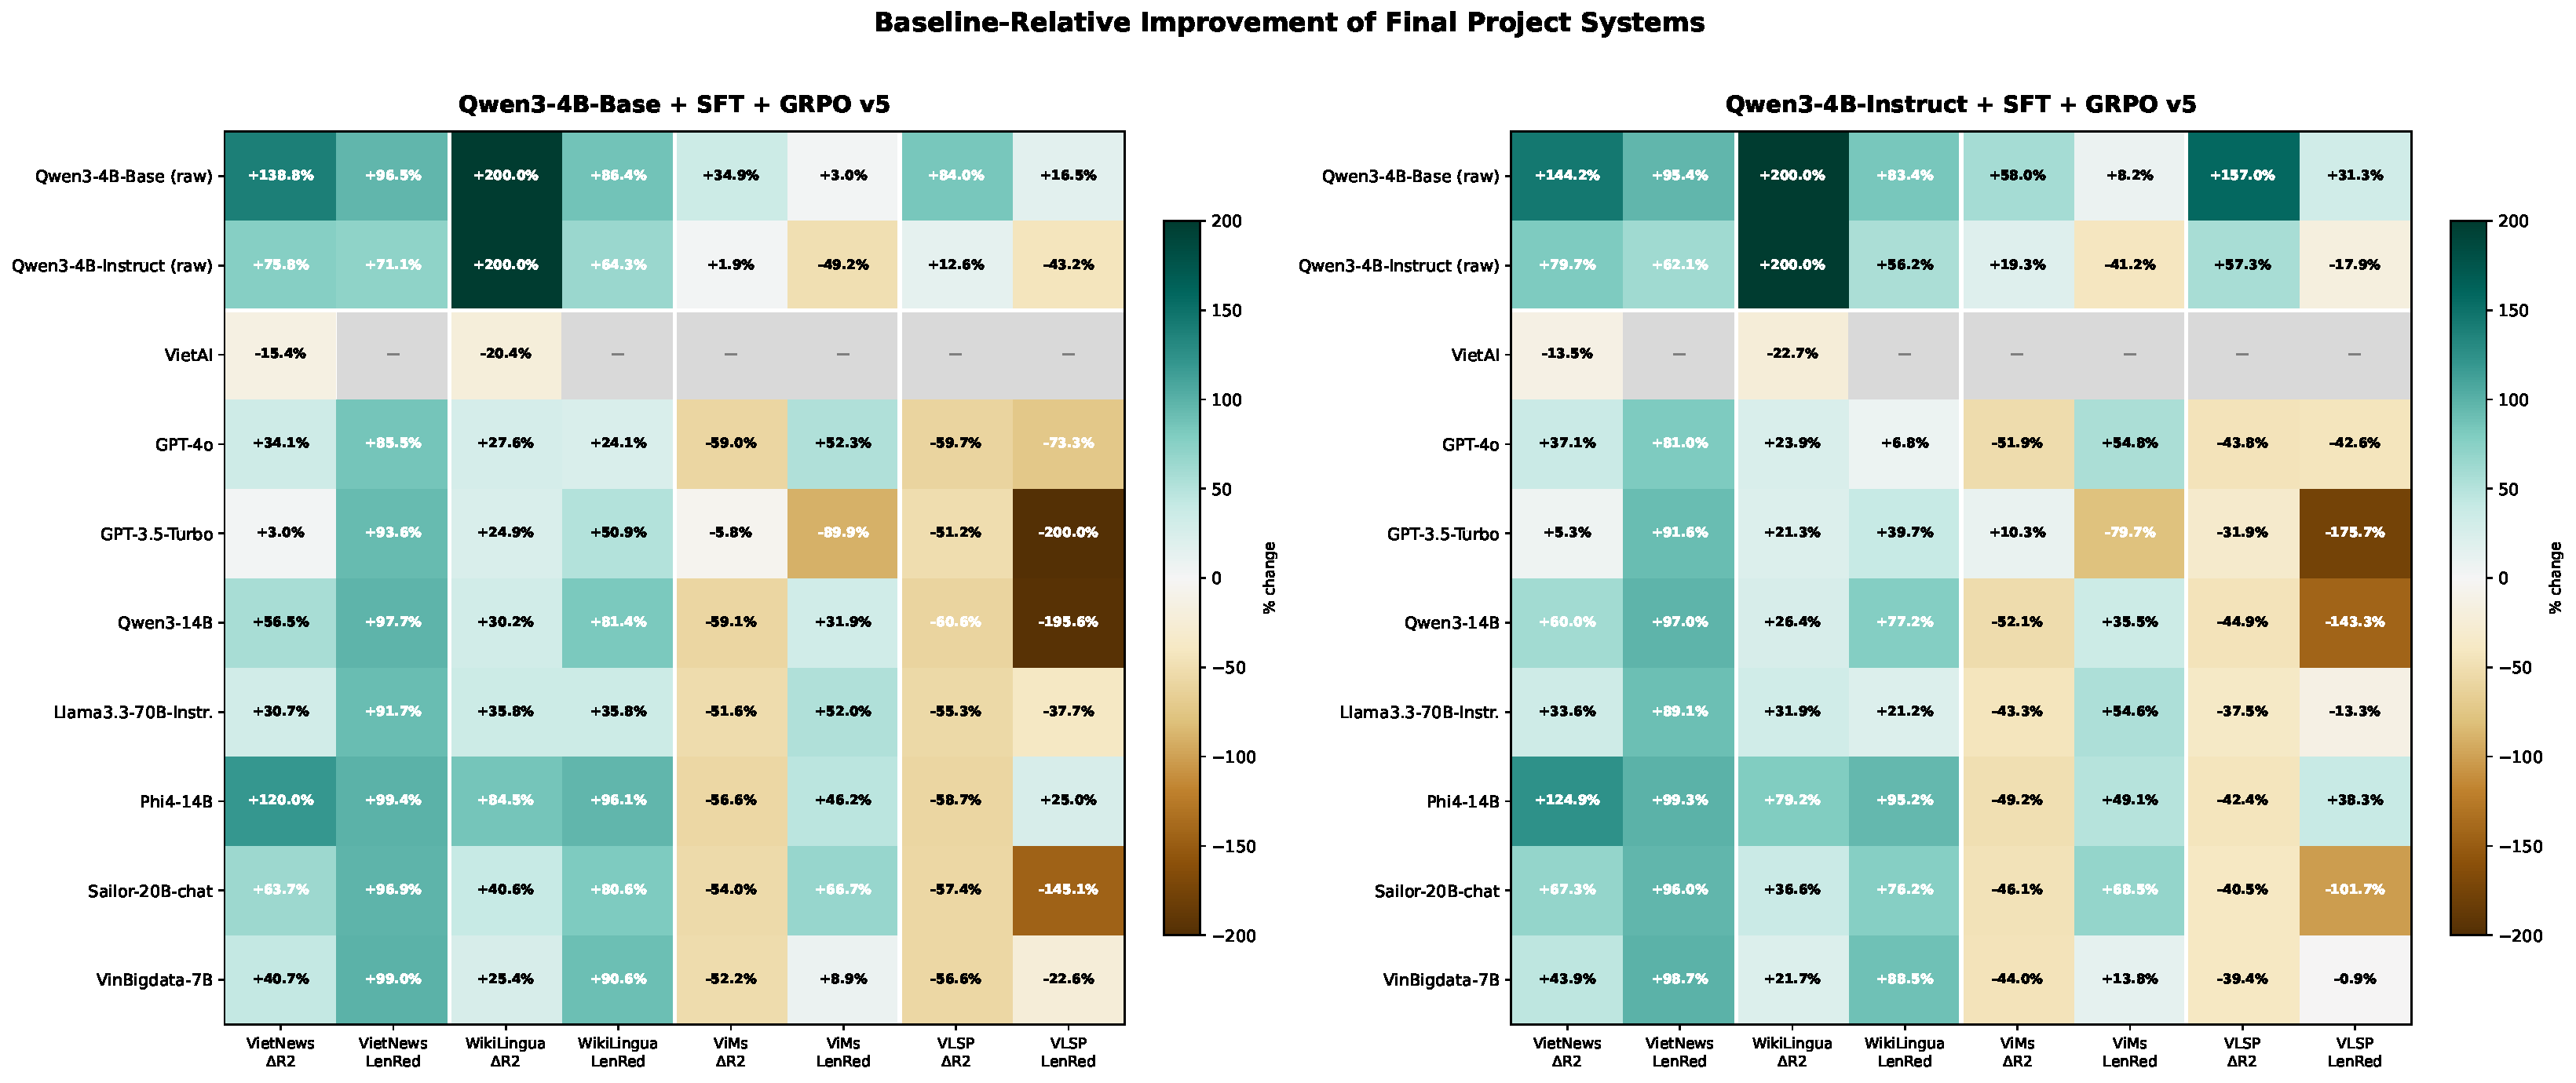
\includegraphics[width=\textwidth]{figures/section52_tradeoff.pdf}
\caption{Baseline-relative improvement summary for the two final project systems. Each dataset is shown explicitly as a two-column block: positive $\Delta$R2 means higher ROUGE-2, positive LenRed means smaller absolute summary length distance, and gray cells mark unavailable values. The first two rows are raw Qwen3-4B baselines, followed by external baselines. Cell text shows the exact percentage change, while color intensity is clipped for readability.}
\label{fig:benchmark-improvement}
\end{figure*}

The two main tables show the raw benchmark values, while Figure~\ref{fig:benchmark-improvement} makes the comparison direction explicit.
On VietNews and WikiLingua, both final systems improve strongly over the raw Qwen3 baselines and over every external baseline with available length-control values; the only ROUGE-2 exception is VietAI, which remains about 18\% higher but does not report matching length-distance values.
The same figure also shows that the method is not merely beating unrelated baselines: relative to the raw Qwen3 backbones, both final systems make especially large ROUGE-2 gains on WikiLingua and strong length-distance reductions on both single-document datasets.

ViMs and VLSP remain visible rather than hidden.
Figure~\ref{fig:benchmark-improvement} shows that both final systems still improve over the raw Qwen3 baselines on ViMs and VLSP ROUGE-2, but they remain substantially below the strongest external multi-document baselines such as GPT-4o and Qwen3-14B on that metric.
The ViMs/VLSP length-control picture is mixed rather than uniformly positive, especially for the Instruct branch against stronger baselines.
Appendix Table~\ref{tab:appendix-benchmark-exploratory} retains the full baseline-relative percentage comparison for readers who want the detailed ViMs/VLSP view.

Between the two backbone instantiations, the Instruct branch is the stronger content model overall, winning ROUGE-2 on VietNews, ViMs, and VLSP.
The Base branch is slightly stronger on WikiLingua ROUGE-2 and also yields the best single-document length distance, especially on WikiLingua.
This is why the paper keeps both final rows in the main benchmark rather than collapsing the method to one backbone only.

\subsection{Within-project Stage-wise Ablation}
Table~\ref{tab:stage-ablation} compresses the internal project comparison into one stage-wise ablation over the two held-out single-document datasets.
Its purpose is to analyze why a two-stage post-training pipeline (SFT + GRPO v5) is necessary and why it represents the optimal configuration compared to SFT-only, Pretrained-only, and Fresh-GRPO variants.
To better visualize this multi-stage interaction on the primary dual objectives—retaining content quality while enforcing a strict length budget—we plot the joint ROUGE-2 and absolute summary length distance trajectory in Figure~\ref{fig:stage-ablation-trajectory}.

\begin{figure*}[t]
\centering
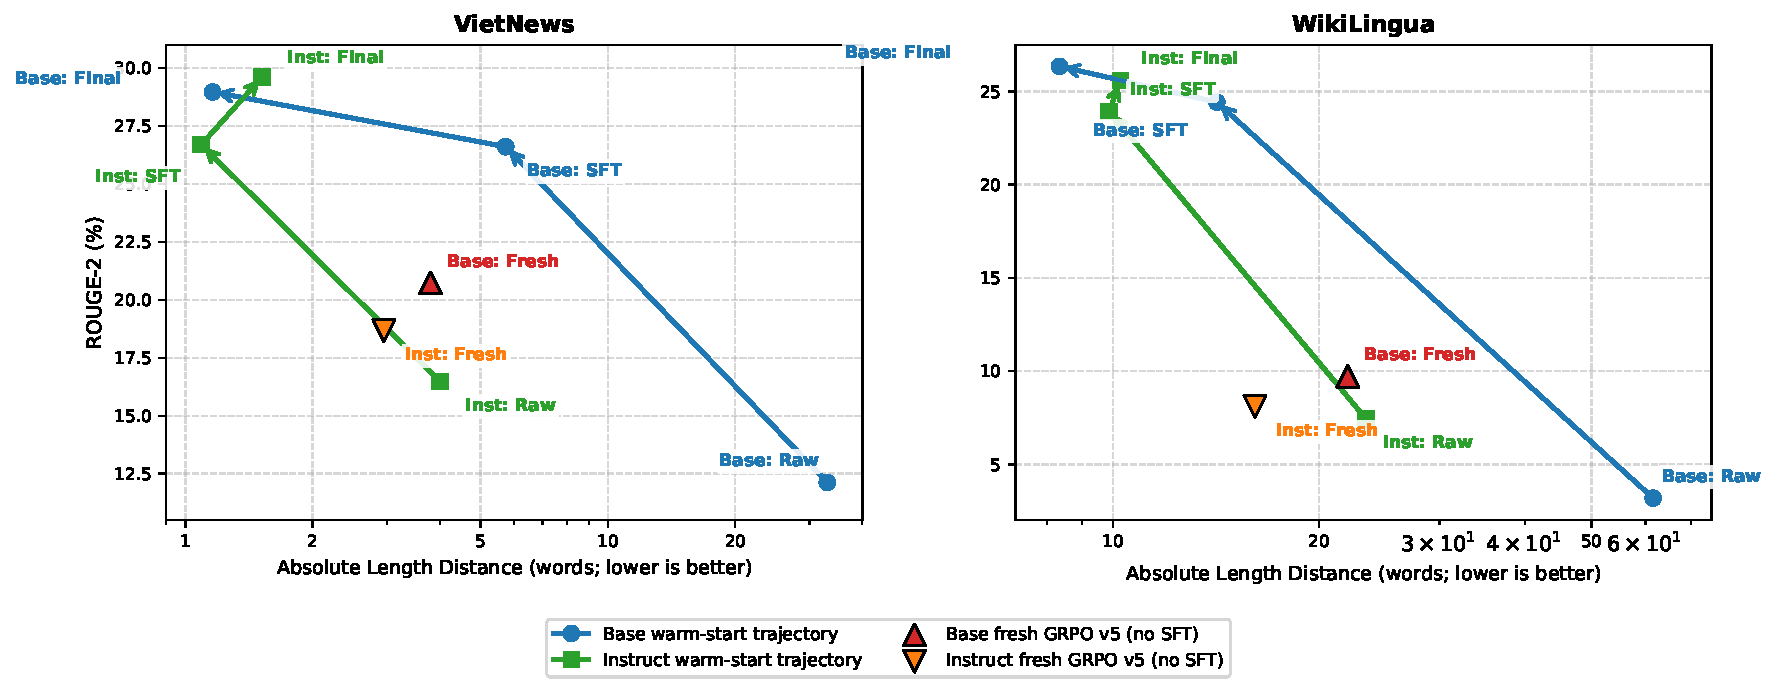
\includegraphics[width=0.95\textwidth]{figures/section53_ablation.pdf}
\caption{Two-panel trade-off trajectory showing ROUGE-2 versus absolute summary length distance for the Base and Instruct backbones on VietNews (left) and WikiLingua (right). Moving towards the top-right corresponds to the optimal region (high-fidelity length control with high-quality content). Arrowed lines display the two-stage post-training progress (Raw $\rightarrow$ SFT $\rightarrow$ SFT+GRPO v5), while standalone markers highlight the performance collapse of Fresh GRPO v5 when SFT initialization is omitted.}
\label{fig:stage-ablation-trajectory}
\end{figure*}

\begin{table*}[t]
\centering
\small
\resizebox{\textwidth}{!}{%
\begin{tabular}{L{0.28\textwidth}cccc}
\toprule
Model & VietNews ROUGE-2 & WikiLingua ROUGE-2 & VietNews LenDist & WikiLingua LenDist \\
\midrule
Base pretrained & 12.13 & 3.18 & 33.03 & 61.59 \\
Base + SFT & 26.61 & 24.43 & 5.73 & 14.18 \\
Base + fresh GRPO v5 & 20.73 & 9.71 & 3.80 & 22.03 \\
Base + SFT + GRPO v5 & \second{28.97} & \best{26.35} & \second{1.16} & \best{8.35} \\
Instruct pretrained & 16.48 & 7.44 & 4.01 & 23.42 \\
Instruct + SFT & 26.70 & 23.93 & \best{1.09} & \second{9.87} \\
Instruct + fresh GRPO v5 & 18.67 & 8.09 & 2.95 & 16.12 \\
Instruct + SFT + GRPO v5 & \best{29.62} & \second{25.59} & 1.52 & 10.25 \\
\bottomrule
\end{tabular}}
\caption{Compact within-project ablation on the two held-out single-document datasets. This table is included to explain the chosen training recipe, not as the paper's headline leaderboard.}
\label{tab:stage-ablation}
\end{table*}

The stage-wise trajectory analysis reveals three critical experimental insights that justify our final pipeline design:

\paragraph{The synergy of bootstrapping (SFT) and refinement (GRPO).}
The baseline pretrained backbones are completely incapable of producing coherent controllable summaries, as shown by their low ROUGE-2 scores and massive length deviations. 
SFT acts as an indispensable first stage: a \textit{content-formatting bootstrap}. 
SFT teaches the model how to follow instruction structures, summarize salient content in fluent Vietnamese, and establish a baseline sensitivity to length prompts.
But SFT alone is not enough; the models still overshoot or undershoot their budgets by an average of $5.73$ to $14.18$ words, because standard cross-entropy loss over text sequences struggles to align strict numerical budgets.
GRPO v5 then acts as an \textit{alignment refiner}. 
Rather than trading off content for length control, GRPO v5 actively improves \textit{both} metrics. 
For instance, on the Base backbone, GRPO refinement reduces length deviation on VietNews by 80\% (from $5.73$ down to a near-perfect $1.16$ words), while simultaneously boosting ROUGE-2 by $2.36\%$ (from $26.61\%$ to $28.97\%$). This demonstrates that GRPO learns to align length constraints by filtering redundant lexical padding, which refines output conciseness and boosts information density.

\paragraph{The failure of Fresh GRPO and the gating reward function.}
Attempting reinforcement learning directly on the pretrained model (Fresh GRPO v5, without the intermediate SFT step) fails catastrophically. 
As shown by the isolated markers in Figure~\ref{fig:stage-ablation-trajectory}, the Fresh GRPO models remain severely bottlenecked on content quality (achieving only $20.73$ and $18.67$ ROUGE-2 on VietNews). 
This behavior is a direct consequence of our multiplicative reward structure, $R_{\text{total}} = R_{\text{acc}} \times (1 + 0.3 R_{\text{len}} + 0.2 R_{\text{sent}})$. 
Without the SFT stage to boot-strap language capabilities, the model's random rollouts during GRPO training consist of empty or degenerate text, resulting in $R_{\text{acc}} = 0$. 
This zeros out the entire reward, preventing the optimization algorithm from receiving any meaningful gradient signal. 
SFT pre-training is therefore a prerequisite to seed the action space with candidates that can pass our quality-gating checks.

\paragraph{Optimal Pareto Frontier and Backbone Choice.}
The trajectory curves in Figure~\ref{fig:stage-ablation-trajectory} visualize the two-stage warm-start as a clear shift towards the top-right corner.
For the Base branch, the absolute length distance decreases by $89.9\%$ on the macro average ($47.31$ words to $4.76$ words) coupled with a $+261.3\%$ relative gain in macro ROUGE-2.
For the Instruct branch, macro length distance is slashed by $57.1\%$ ($13.72$ to $5.89$ words) alongside a $+130.8\%$ relative macro ROUGE-2 gain.
By comparing both trajectories, we see that the Instruct-initialized pipeline represents the ultimate content capability model (achieving the highest overall ROUGE-2 of $29.62$ on VietNews), whereas the Base-initialized pipeline yields the most remarkable relative progress and matches or even slightly exceeds the Instruct model's length-control accuracy (reaching the lowest single-dataset deviation of $1.16$ words).
This confirms that our two-stage bootstrapped recipe is highly robust across different foundational starting points.

\subsection{Reward-hacking Mitigation Ablation}
The v3-to-v5 comparison is a package-level failure analysis rather than a claim about one detector or one hyperparameter in isolation.
Nevertheless, the stored artefacts show a clear stabilization story for the branches that were previously most brittle.

\begin{table*}[t]
\centering
\small
\resizebox{\textwidth}{!}{%
\begin{tabular}{L{0.24\textwidth}ccccc}
\toprule
Run & ROUGE-2 & LenErr\% & Deg.\% & $R_{\text{acc}}=0$\% & Mean $R_{\text{acc}}$ \\
\midrule
Base fresh v3 & 10.58 & 163.16 & 23.81 & 27.16 & 0.1854 \\
Base fresh v5 & 18.66 & 29.05 & 0.32 & 1.94 & 0.3160 \\
Base SFT-init v3 & 18.03 & 425.00 & 14.77 & 1.16 & 0.2508 \\
Base SFT-init v5 & \second{26.38} & \best{14.94} & 2.71 & \best{0.45} & \second{0.4009} \\
Instruct fresh v3 & 15.00 & 30.08 & \best{0.03} & 1.48 & 0.2768 \\
Instruct fresh v5 & 16.69 & 22.78 & \second{0.03} & 1.58 & 0.2979 \\
Instruct SFT-init v3 & 25.06 & 19.94 & 0.94 & 1.19 & 0.3837 \\
Instruct SFT-init v5 & \best{27.65} & \second{15.85} & 1.42 & \second{0.45} & \best{0.4213} \\
\bottomrule
\end{tabular}}
\caption{Reward-hacking mitigation ablation from v3 to v5. All values are recomputed from stored generations with the current reward implementation.}
\label{tab:reward-mitigation}
\end{table*}

As shown in Table~\ref{tab:reward-mitigation}, Base fresh is the clearest recovery case: its degenerate rate falls from 23.81\% to 0.32\%, its zero-content rate falls from 27.16\% to 1.94\%, and its ROUGE-2 rises from 10.58 to 18.66.
Base SFT-init v3 is less visibly degenerate but still fails through severe length explosion; v5 cuts its relative length error from 425.00\% to 14.94\% while raising ROUGE-2 from 18.03 to 26.38.
The Instruct branches were already more stable, so their v3-to-v5 gains are smaller, but they still support the choice of the final package.

\subsection{V4-to-V5 Configuration-bundle Ablation}
The v4 and v5 comparisons should be interpreted as bundle-level operating points rather than isolated hyperparameter ablations.
Table~\ref{tab:v4v5} therefore uses macro averages over the two held-out single-document datasets only.

\begin{table*}[t]
\centering
\small
\resizebox{\textwidth}{!}{%
\begin{tabular}{L{0.20\textwidth}rrrrrr}
\toprule
Branch & v4 ROUGE-2 & v5 ROUGE-2 & v4 LenErr\% & v5 LenErr\% & v4 LenDist & v5 LenDist \\
\midrule
Base fresh & 10.93 & 15.22 & 91.67 & 36.65 & 26.70 & 12.90 \\
Base SFT-init & \best{26.25} & \best{27.66} & \second{17.88} & \second{10.56} & \second{7.05} & \second{4.80} \\
Instruct fresh & 12.39 & 13.38 & 33.98 & 27.88 & 11.65 & 9.50 \\
Instruct SFT-init & \second{26.23} & \second{27.60} & \best{13.09} & \best{13.68} & \best{6.00} & \best{5.85} \\
\bottomrule
\end{tabular}}
\caption{Configuration-bundle ablation from v4 to v5 on VietNews and WikiLingua macro averages. The table supports the choice of v5 as the canonical GRPO setting, but it does not isolate any single hyperparameter.}
\label{tab:v4v5}
\end{table*}

As shown in Table~\ref{tab:v4v5}, the clearest gains appear in the fresh branches, where v5 improves both ROUGE-2 and length-control metrics.
For the stronger SFT-initialized branches, v5 is still the better overall operating point: it improves both metrics for Base SFT-init and improves ROUGE-2 plus absolute length distance for Instruct SFT-init, even though relative length error is nearly tied.

\section{Conclusion}
This paper reframes the project as a method-first study of lightweight post-training for controllable Vietnamese summarization.
The central result is that a two-stage recipe, combining instruction-conditioned LoRA-SFT with custom GRPO v5, produces strong single-document performance when evaluated with both ROUGE-2 and absolute summary length distance.
In the main benchmark, the final project systems outperform most contextual large-model baselines on VietNews and WikiLingua, while also maintaining much tighter length control.

The ablations explain why the final report should focus on SFT + GRPO v5.
SFT is the dominant improvement stage, fresh GRPO is not a substitute for supervised instruction tuning, and the v3-to-v5 mitigation package sharply reduces failure-prone behavior in the branches that were previously unstable.
The v4-to-v5 comparison further supports v5 as the most reliable bundle among the stored GRPO configurations.

At the same time, the paper keeps its claim boundary explicit.
VietNews and WikiLingua are the only datasets that support strong held-out conclusions, ViMs and VLSP remain exploratory because of split overlap, and the external baseline rows are contextual rather than protocol-matched reruns.
The main takeaway is therefore narrow but useful: the present SFT + GRPO v5 pipeline is a credible and efficient recipe for single-document controllable Vietnamese summarization, while multi-document generalization remains future work.

\clearpage
\appendix
\onecolumn

\section{Appendix}
\label{sec:appendix}

\subsection{Full Within-project Variant Tables}
\label{sec:appendix-variants}
Tables~\ref{tab:appendix-rouge}--\ref{tab:appendix-lenerr} provide the full four-dataset view for all canonical Qwen3 project variants.
These tables are retained as internal context, but they are not the headline benchmark of the paper.

\begin{table}[H]
\centering
\small
\resizebox{\linewidth}{!}{%
\begin{tabular}{L{0.34\linewidth}cccc}
\toprule
Model & VietNews & WikiLingua & ViMs\explore & VLSP\explore \\
\midrule
Base pretrained & 12.13 & 3.18 & 13.46 & 9.49 \\
Base + SFT & 26.61 & 24.43 & \best{25.65} & \best{28.14} \\
Base + fresh GRPO v5 & 20.73 & 9.71 & 20.28 & 18.14 \\
Base + SFT + GRPO v5 & \second{28.97} & \best{26.35} & 18.16 & 17.46 \\
Instruct pretrained & 16.48 & 7.44 & 17.83 & 15.51 \\
Instruct + SFT & 26.70 & 23.93 & \second{24.71} & \second{27.03} \\
Instruct + fresh GRPO v5 & 18.67 & 8.09 & 18.43 & 16.05 \\
Instruct + SFT + GRPO v5 & \best{29.62} & \second{25.59} & 21.27 & 24.39 \\
\bottomrule
\end{tabular}}
\caption{ROUGE-2 (\%) across all four datasets for the canonical Qwen3 project variants.}
\label{tab:appendix-rouge}
\end{table}

\begin{table}[H]
\centering
\small
\resizebox{\linewidth}{!}{%
\begin{tabular}{L{0.34\linewidth}cccc}
\toprule
Model & VietNews & WikiLingua & ViMs\explore & VLSP\explore \\
\midrule
Base pretrained & 33.03 & 61.59 & 92.01 & 120.33 \\
Base + SFT & 5.73 & 14.18 & 66.45 & \second{61.64} \\
Base + fresh GRPO v5 & 3.80 & 22.03 & 71.77 & 88.02 \\
Base + SFT + GRPO v5 & \second{1.16} & \best{8.35} & 89.23 & 100.50 \\
Instruct pretrained & 4.01 & 23.42 & \best{59.80} & 70.17 \\
Instruct + SFT & \best{1.09} & \second{9.87} & 64.55 & \best{62.22} \\
Instruct + fresh GRPO v5 & 2.95 & 16.12 & \second{63.05} & 72.91 \\
Instruct + SFT + GRPO v5 & 1.52 & 10.25 & 84.45 & 82.71 \\
\bottomrule
\end{tabular}}
\caption{Absolute summary length distance across all four datasets for the canonical Qwen3 project variants.}
\label{tab:appendix-lendist}
\end{table}

\begin{table}[H]
\centering
\small
\resizebox{\linewidth}{!}{%
\begin{tabular}{L{0.34\linewidth}cccc}
\toprule
Model & VietNews & WikiLingua & ViMs\explore & VLSP\explore \\
\midrule
Base pretrained & 205.89 & 174.67 & 42.61 & 47.93 \\
Base + SFT & 31.19 & 24.72 & 38.69 & 27.53 \\
Base + fresh GRPO v5 & 22.36 & 50.94 & 31.89 & 34.33 \\
Base + SFT + GRPO v5 & \second{6.43} & \best{14.69} & 44.42 & 42.55 \\
Instruct pretrained & 24.50 & 57.47 & \best{26.07} & \second{27.09} \\
Instruct + SFT & \best{6.26} & 18.34 & 31.55 & \best{24.51} \\
Instruct + fresh GRPO v5 & 17.08 & 38.67 & \second{28.37} & 28.76 \\
Instruct + SFT + GRPO v5 & 9.24 & \second{18.11} & 39.14 & 32.85 \\
\bottomrule
\end{tabular}}
\caption{Relative length error (\%) across all four datasets for the canonical Qwen3 project variants.}
\label{tab:appendix-lenerr}
\end{table}

\subsection{Exploratory Multi-document Baseline Comparison}
\label{sec:appendix-exploratory}
Table~\ref{tab:appendix-benchmark-exploratory} keeps the full baseline-relative comparison on ViMs and VLSP.
It is retained in the appendix because it is useful diagnostic context, but it should not dominate the main method-first narrative of the paper.

\begin{table}[H]
\centering
\small
\resizebox{\linewidth}{!}{%
\begin{tabular}{L{0.30\linewidth}cccc}
\toprule
Baseline &
\multicolumn{2}{c}{Qwen3-4B-Base + SFT + GRPO v5} &
\multicolumn{2}{c}{Qwen3-4B-Instruct + SFT + GRPO v5} \\
\cmidrule(lr){2-3} \cmidrule(lr){4-5}
& $\Delta$ ROUGE-2$\uparrow$ & LenDist reduction$\uparrow$ & $\Delta$ ROUGE-2$\uparrow$ & LenDist reduction$\uparrow$ \\
\midrule
VietAI & -- & -- & -- & -- \\
GPT-4o & -59.4\% & +22.6\% & -47.9\% & +31.8\% \\
GPT-3.5-Turbo & \best{-35.3\%} & -146.4\% & \best{-17.1\%} & -117.1\% \\
Qwen3-14B & -59.8\% & -15.0\% & -48.5\% & -1.3\% \\
Llama3.3-70B-Instruct & \second{-53.5\%} & +26.7\% & \second{-40.4\%} & +35.5\% \\
Phi4-14B & -57.7\% & \second{+36.8\%} & -45.7\% & \second{+44.3\%} \\
Sailor-20B-chat & -55.7\% & \best{+38.6\%} & -43.2\% & \best{+45.9\%} \\
VinBigdata (7B) & -54.5\% & -5.4\% & -41.6\% & +7.1\% \\
\bottomrule
\end{tabular}}
\caption{Exploratory relative change against each contextual baseline on the ViMs and VLSP macro average. Positive values are better for both columns, but the table is diagnostic only because both datasets overlap with project training or validation pools.}
\label{tab:appendix-benchmark-exploratory}
\end{table}

\subsection{Sentence-control Results}
\label{sec:appendix-sentence}
Sentence-control results are retained here because the main paper focuses on ROUGE-2 and absolute summary length distance.

\begin{table}[H]
\centering
\small
\resizebox{\linewidth}{!}{%
\begin{tabular}{L{0.26\linewidth}cccccc}
\toprule
Model & VN Exact\% & VN Tol.\% & VN MAE & WL Exact\% & WL Tol.\% & WL MAE \\
\midrule
Base pretrained & 73.95 & 89.55 & 0.550 & 15.4 & 32.4 & 2.910 \\
Base + SFT & 91.40 & 96.55 & 4.299 & 58.6 & 83.8 & 1.674 \\
Base + fresh GRPO v5 & 91.80 & 99.30 & 0.089 & 34.2 & 72.8 & 1.226 \\
Base + SFT + GRPO v5 & 93.85 & 98.75 & 0.316 & 65.6 & \second{95.6} & 0.470 \\
Instruct pretrained & 93.95 & \second{99.40} & 0.067 & 34.2 & 64.6 & 1.582 \\
Instruct + SFT & \second{95.45} & 98.90 & 0.058 & \best{88.0} & 97.0 & 0.204 \\
Instruct + fresh GRPO v5 & 94.85 & \best{99.60} & \second{0.056} & 46.8 & 72.4 & 1.178 \\
Instruct + SFT + GRPO v5 & \best{96.95} & 99.05 & \best{0.041} & \second{78.8} & 95.6 & \second{0.340} \\
\bottomrule
\end{tabular}}
\caption{Sentence-control metrics recomputed from stored generations. ``Tol.'' counts a prediction as correct when the sentence count is within $\pm 1$ of the requested budget.}
\label{tab:appendix-sentence}
\end{table}

\subsection{Dataset Processing Details}
\label{sec:appendix-processing}
The final JSONL artefacts are produced by the project's data processing and augmentation modules.
The most important preprocessing rules are listed below.

\begin{itemize}
    \item Shared preprocessing truncates sources to 8,000 characters and summaries to 1,500 characters, then replaces underscore-based segmentation markers with spaces.
    \item VietNews uses the first line of each file as the target headline, the sapo plus body as source text, and drops the last line as caption-like trailing content.
    \item WikiLingua flattens \textit{src} and \textit{tgt} sentence lists into single strings.
    \item ViMs reads each document in a cluster and concatenates the documents into a single source with explicit boundary markers.
    \item VLSP flattens each cluster in the same style, prefers the abstractive \textit{summary} field, and falls back to label-based extraction only when a summary is unavailable.
    \item SFT and GRPO intentionally use different training pools: SFT filters short VietNews titles and excludes VLSP, while GRPO keeps all VietNews and includes VLSP.
\end{itemize}

\subsection{Pipeline Configurations and Prompt Templates}
\label{sec:appendix-prompts}
This subsection summarizes the end-to-end pipeline configuration used by the paper.
The source of truth is the project's canonical configuration files, training scripts, evaluation pipeline, and audit documentation.
Prompt examples are shown with full Vietnamese diacritics and follow the instruction format used throughout the pipeline.

\paragraph{Data augmentation and prompt construction.}
\begin{table}[H]
\centering
\small
\begin{tabular}{L{0.17\linewidth}L{0.20\linewidth}L{0.28\linewidth}L{0.25\linewidth}}
\toprule
Process & Prompt shape & Template policy & Stored outputs \\
\midrule
SFT & system + user + assistant & Always uses the approximate control template family & \textit{messages} plus \textit{meta} \\
GRPO train/val & system + user & Rotates three length templates and three sentence templates across prompts & \textit{prompt}, \textit{reference}, and \textit{meta} \\
Evaluation/test & system + user & Deterministic test prompt; \textit{make\_test\_prompt()} fixes template index 0 & \textit{prompt}, \textit{reference}, and \textit{meta} \\
\bottomrule
\end{tabular}
\caption{Prompt-construction rules used by the pipeline.}
\label{tab:appendix-prompt-rules}
\end{table}

\begin{table}[H]
\centering
\small
\begin{tabular}{L{0.18\linewidth}L{0.34\linewidth}L{0.34\linewidth}}
\toprule
Signal & Template families & Notes \\
\midrule
Length & \textit{khoang X tu}; \textit{trong khoang lo-hi tu}; \textit{khong qua X tu} & SFT uses only the first form; GRPO rotates all three; eval fixes the first form \\
Sentence & \textit{khoang X cau}; \textit{trong khoang lo-hi cau}; \textit{khong qua X cau} & Same rotation policy as the length templates \\
\bottomrule
\end{tabular}
\caption{Control-template families generated by \textit{PromptAugmenter}.}
\label{tab:appendix-template-families}
\end{table}

All prompt-bearing samples preserve metadata for the reward functions and analysis logs.
The core fields are \textit{target\_length}, \textit{target\_sentences}, \textit{length\_requirement}, and \textit{sentence\_requirement}; the pipeline also tracks source and target length statistics such as \textit{source\_length}.

\paragraph{Canonical SFT configuration.}
\begin{table}[H]
\centering
\small
\begin{tabular}{L{0.34\linewidth}L{0.56\linewidth}}
\toprule
Setting & Canonical paper configuration \\
\midrule
Backbone family & Qwen3-4B-Base or Qwen3-4B \\
LoRA adapter & $r = 32$, $\alpha = 32$, dropout $0.05$; target modules \textit{q/k/v/o\_proj} and \textit{gate/up/down\_proj} \\
Sequence length & $3072$ on H200/A100; $2048$ on V100 \\
Training & $\mathit{lr} = 5\times10^{-5}$, cosine scheduler, $\mathit{warmup\_ratio} = 0.1$, $\textit{epochs} = 2.0$ \\
Thinking suppression & $\mathit{disable\_thinking} = \text{True}$ \\
Batch calibration & Enabled before training \\
Checkpoint behavior & Model-family-specific output directory; resume from latest checkpoint when present \\
\bottomrule
\end{tabular}
\caption{Canonical SFT configuration used by the paper.}
\label{tab:appendix-sft-config}
\end{table}

\begin{table}[H]
\centering
\small
\begin{tabular}{lccc}
\toprule
GPU tier & Start batch & Grad. accum. & Effective batch \\
\midrule
H200 & 10 & 2 & 20 \\
A100 & 6 & 3 & 18 \\
V100 & 2 & 4 & 8 \\
\bottomrule
\end{tabular}
\caption{SFT per-GPU starting presets used in the canonical training runs. Auto-calibration can adjust these values at runtime.}
\label{tab:appendix-sft-gpu}
\end{table}

The appendix tables intentionally follow the launch-script presets rather than the raw library defaults, because the launch scripts are the source of truth for the canonical paper runs.

\paragraph{Canonical GRPO v5 configuration.}
\begin{table}[H]
\centering
\small
\begin{tabular}{L{0.34\linewidth}L{0.56\linewidth}}
\toprule
Setting & Canonical paper configuration \\
\midrule
Initialization & SFT-initialized warm start \\
Core v5 hyperparameters & $K = 8$, $\mathit{lr} = 2\times10^{-6}$, $\beta = 0.04$, $\mathit{total\_steps} = 800$ \\
Rollout decoding & $\mathit{temperature} = 0.7$, $\mathit{top\_p} = 0.9$, $\mathit{do\_sample} = \text{True}$, $\mathit{max\_new\_tokens} = 80$, $\mathit{max\_seq\_length} = 3072$ \\
Reward weights & Accuracy $0.5$, length $0.3$, sentence $0.2$ \\
Stability settings & $\mathit{gradient\_checkpointing} = \text{True}$, $\mathit{disable\_thinking} = \text{True}$, auto-calibration enabled \\
Repetition controls & $\mathit{repetition\_penalty} = 1.0$, $\mathit{no\_repeat\_ngram\_size} = 0$ \\
\bottomrule
\end{tabular}
\caption{Canonical GRPO v5 configuration used in the main paper results.}
\label{tab:appendix-grpo-config}
\end{table}

\begin{table}[H]
\centering
\small
\begin{tabular}{lccc}
\toprule
GPU tier & Start batch & Grad. accum. & Effective prompts/update \\
\midrule
H200 & 4 & 4 & 16 \\
A100 & 2 & 8 & 16 \\
V100 & 1 & 16 & 16 \\
\bottomrule
\end{tabular}
\caption{GRPO per-GPU starting presets used in the canonical training runs. Auto-calibration can refine these values at runtime.}
\label{tab:appendix-grpo-gpu}
\end{table}

For reference only, the main ablation bundle changes are \textit{v4}: $K=4$, $\mathit{lr} = 5\times10^{-7}$, $\beta = 0.15$; \textit{v3} and \textit{v4} remain ablation settings and should not be read as the canonical appendix configuration.

\paragraph{Evaluation configuration.}
\begin{table}[H]
\centering
\small
\begin{tabular}{L{0.34\linewidth}L{0.56\linewidth}}
\toprule
Setting & Frozen evaluation protocol \\
\midrule
Decoding & $\mathit{temperature} = 0.3$, $\mathit{top\_p} = 0.9$, $\mathit{do\_sample} = \text{True}$, $\mathit{max\_new\_tokens} = 256$ \\
Batching & $\mathit{batch\_size} = 8$ \\
Prompt formatting & $\mathit{apply\_chat\_template(..., enable\_thinking} = \text{False)}$ when supported \\
Prompt truncation & Tokenizer truncates prompts to $3072 - \mathit{max\_new\_tokens}$ \\
Evaluation inputs & Per-dataset test artefacts plus the combined test split \\
Metrics in main paper & ROUGE-2 and Length Distance; sentence-control kept in appendix \\
Randomness & One-shot low-temperature sampling; no saved seed \\
\bottomrule
\end{tabular}
\caption{Frozen evaluation configuration used to generate the paper tables.}
\label{tab:appendix-eval-config}
\end{table}

\noindent\textbf{SFT prompt example.}\par\smallskip
\noindent\colorbox{promptbg}{%
\begin{minipage}{\dimexpr\textwidth-2\fboxsep\relax}
\small\vspace{4pt}
\textbf{System:} Bạn là một trợ lý AI chuyên tóm tắt văn bản tiếng Việt. Hãy tạo ra bản tóm tắt ngắn gọn, chính xác, tuân thủ đúng yêu cầu về độ dài và số câu.

\smallskip
\textbf{User:}
\begin{itemize}
  \item Độ dài: khoảng 22 từ
  \item So cau: khoang 1 cau
\end{itemize}
Van ban: \textless{}source article\textgreater

\smallskip
\textbf{Assistant:}
\textless{}gold summary\textgreater
\vspace{4pt}
\end{minipage}}

\medskip
\noindent\textbf{GRPO rollout prompt example.}\par\smallskip
\noindent\colorbox{promptbg}{%
\begin{minipage}{\dimexpr\textwidth-2\fboxsep\relax}
\small\vspace{4pt}
\textbf{System:} Bạn là một trợ lý AI chuyên tóm tắt văn bản tiếng Việt. Hãy tạo ra bản tóm tắt ngắn gọn, chính xác, tuân thủ đúng yêu cầu về độ dài và số câu.

\smallskip
\textbf{User:}
\begin{itemize}
  \item Do dai: trong khoang 18--26 tu
  \item So cau: trong khoang 1--2 cau
\end{itemize}
Van ban: \textless{}source article\textgreater

\smallskip
\textit{reference} = \textless{}gold summary\textgreater\\
\textit{meta.target\_length} = 22\\
\textit{meta.target\_sentences} = 1\\
\textit{meta.length\_requirement} = ``trong khoang 18--26 tu''\\
\textit{meta.sentence\_requirement} = ``trong khoang 1--2 cau''
\vspace{4pt}
\end{minipage}}

\medskip
\noindent\textbf{Evaluation/test prompt example.}\par\smallskip
\noindent\colorbox{promptbg}{%
\begin{minipage}{\dimexpr\textwidth-2\fboxsep\relax}
\small\vspace{4pt}
\textbf{System:} Bạn là một trợ lý AI chuyên tóm tắt văn bản tiếng Việt. Hãy tạo ra bản tóm tắt ngắn gọn, chính xác, tuân thủ đúng yêu cầu về độ dài và số câu.

\smallskip
\textbf{User:}
\begin{itemize}
  \item Độ dài: khoảng 22 từ
  \item So cau: khoang 1 cau
\end{itemize}
Van ban: \textless{}source article\textgreater

\smallskip
\textit{reference} = \textless{}gold summary\textgreater\\
\textit{meta.dataset} = ``vietnews''
\vspace{4pt}
\end{minipage}}

GRPO training and evaluation share the same prompt shape: both keep only the system and user turns, store the gold summary separately as \textit{reference}, and preserve the control metadata in \textit{meta}.
The differences are that GRPO rotates all template families during rollout training, whereas evaluation fixes the deterministic approximate template, and SFT is the only stage that includes an assistant turn inside the serialized chat sample.

\subsection{No-sentence-reward Ablation}
\label{sec:appendix-nosentence}
The no-sentence ablation is informative but not decisive.
Both sides of the comparison still use sampling without a saved evaluation seed, so the correct conclusion is \emph{inconclusive} rather than a clean causal claim about sentence reward.

\begin{table}[H]
\centering
\small
\begin{tabular}{L{0.26\linewidth}rrrrr}
\toprule
Branch & $w_{\mathrm{sent}}$ & ROUGE-2 & LenErr\% & Sent. Exact\% & Sent. MAE \\
\midrule
Base fresh v4 & 0.2 & 13.88 & 76.44 & 59.42 & \best{1.136} \\
Base fresh ablation & 0.0 & 13.99 & 76.50 & 60.32 & \second{1.163} \\
Base SFT-init v4 & 0.2 & \second{26.71} & \second{20.82} & \second{73.39} & 2.009 \\
Base SFT-init ablation & 0.0 & \best{26.85} & \best{17.21} & \best{73.65} & 1.452 \\
\bottomrule
\end{tabular}
\caption{No-sentence-reward ablation computed from a frozen evaluation snapshot. The differences are too small under the current sampling-based protocol to support a clean causal statement.}
\label{tab:appendix-nosentence}
\end{table}

\bibliography{custom}

\end{document}
